\begin{figure*}[tb]
  \centering
  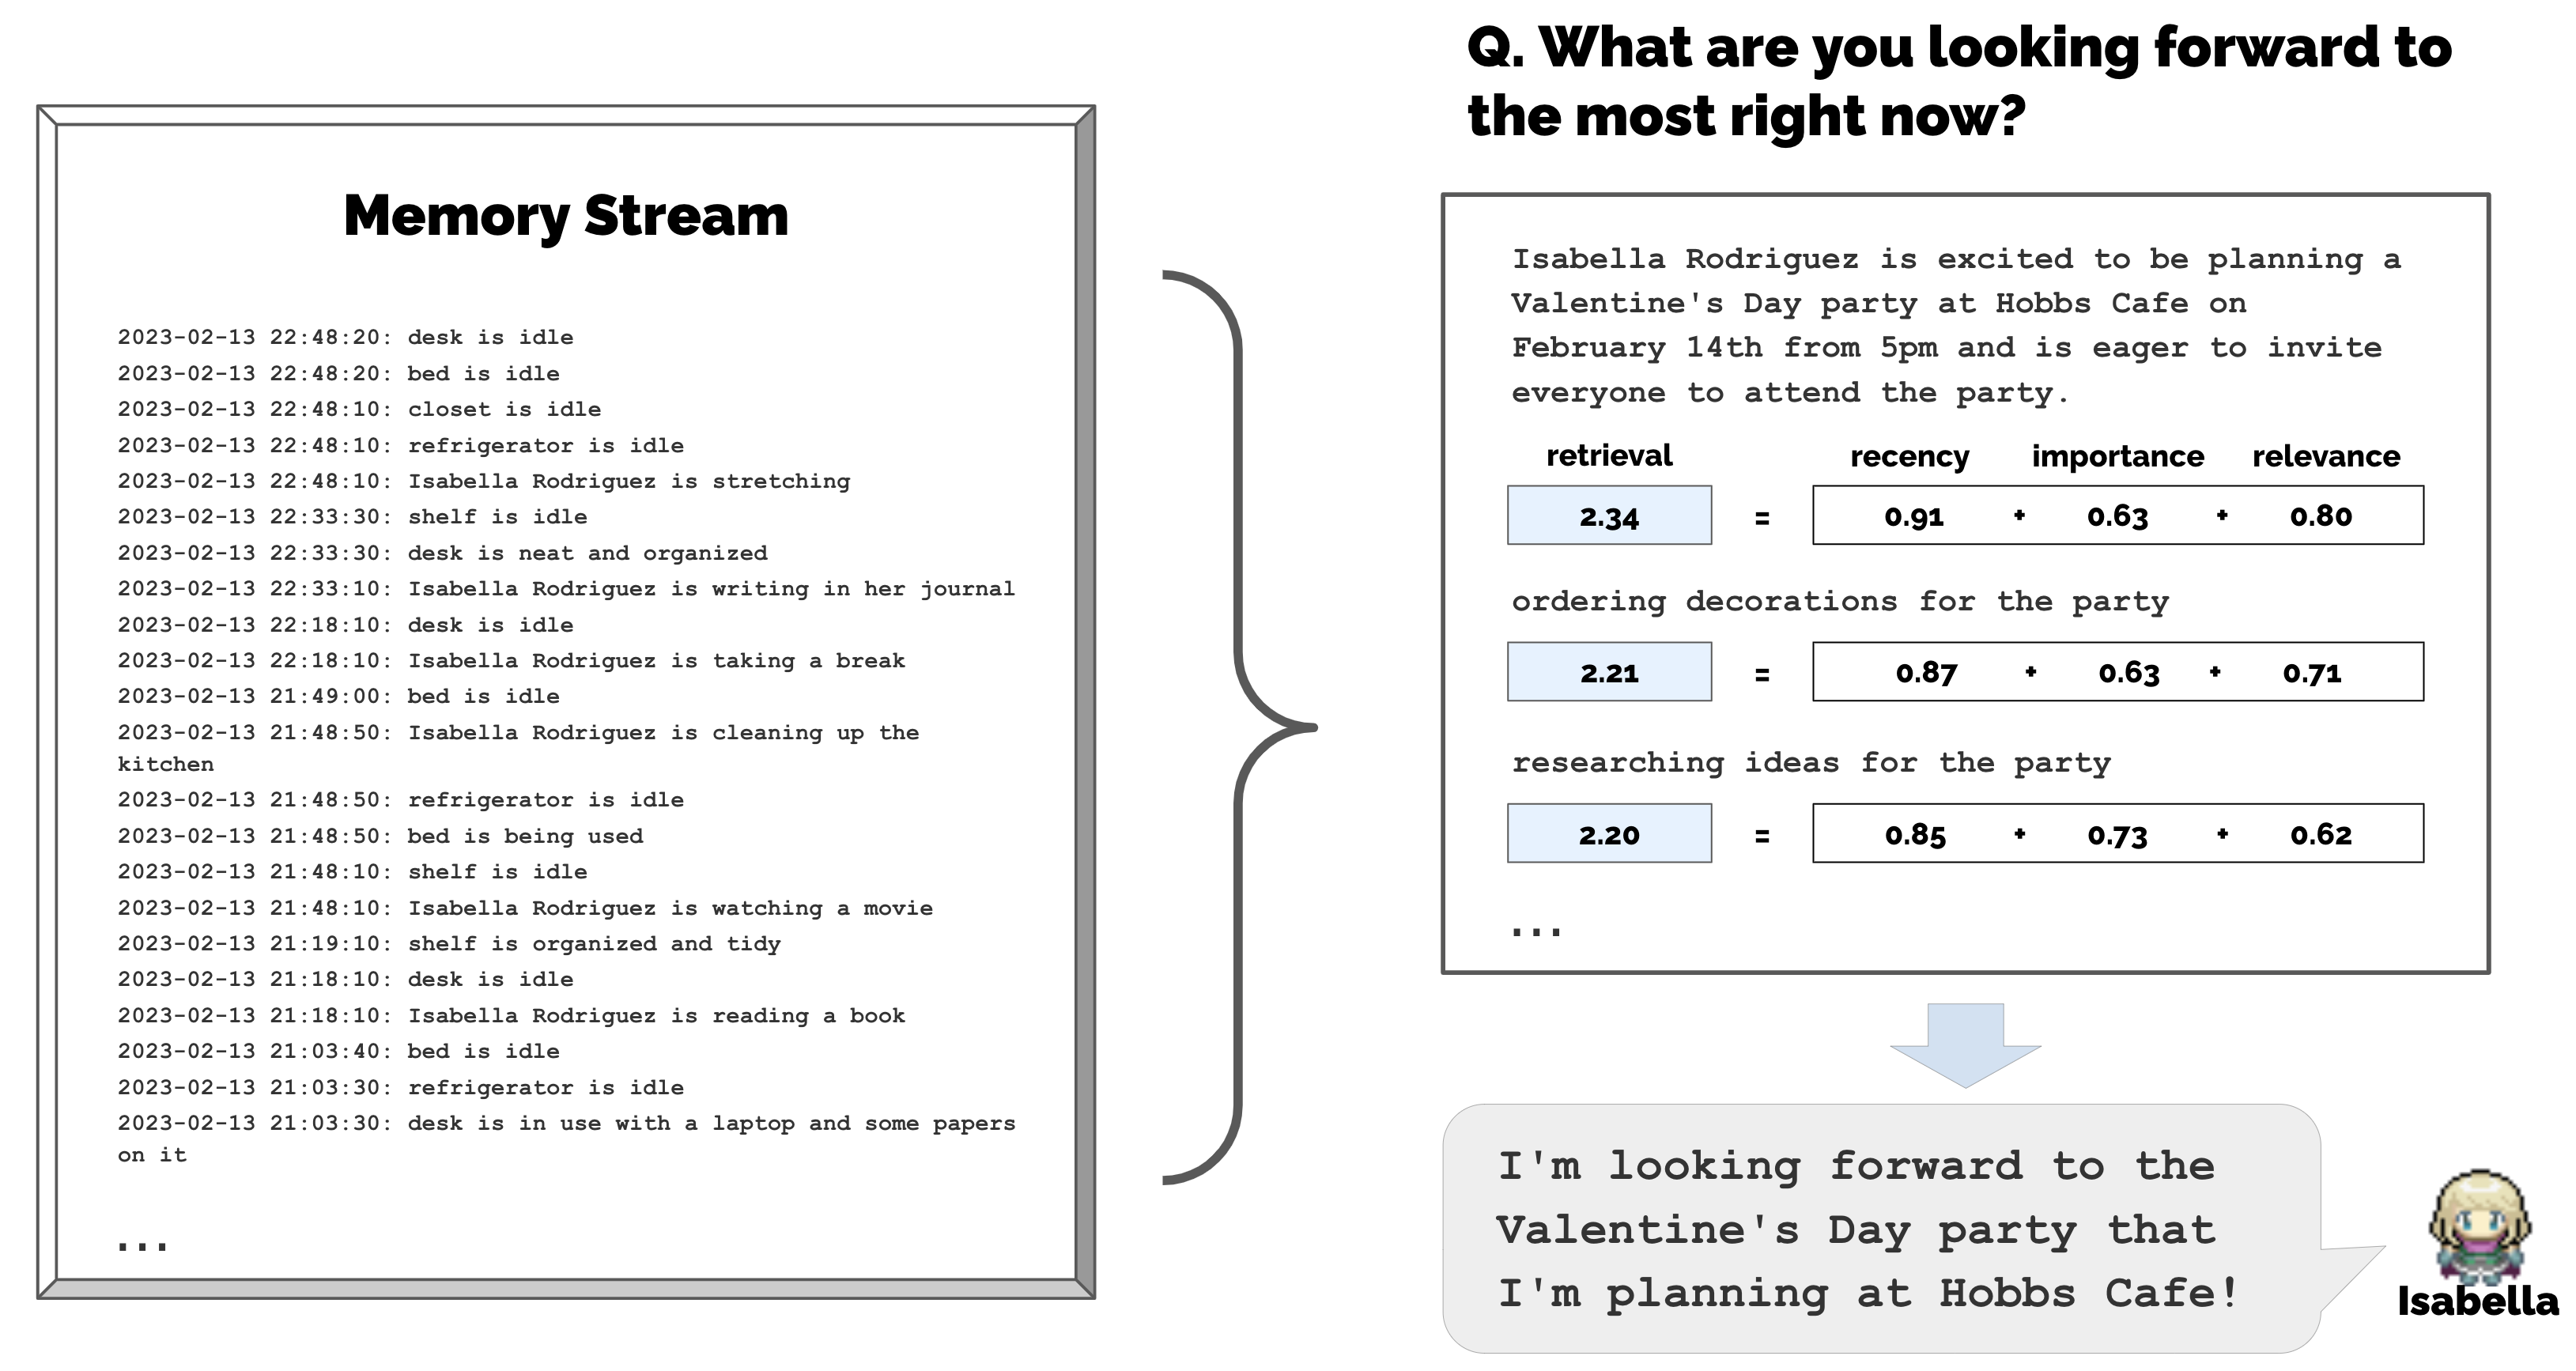
\includegraphics[width=0.86\textwidth]{figures/figure_retrieval2.png}
  \caption{The memory stream comprises a large number of observations that are relevant and irrelevant to the agent's current situation. Retrieval identifies a subset of these observations that should be passed to the language model to condition its response to the situation.}
  \Description{On the left, a large list of events such as ``refrigerator is idle''. On the right, the question ``What are you looking forward to the most right now?'', followed by retrieval calculations that rank ``ordering decorations for the party'' and ``researching ideas for the party'' highly. Based on these memories, Isabella responds, ``I'm looking forward to the Valentine's Day party that I'm planning at Hobbs Cafe!''}
  \label{fig:retrieval_function}
\end{figure*}